\section{Physics Package based on Microwave Optical Double-Resonance (MODR)}

\begin{frame}{$^{87}Rb$ Reference Cell}

    At the heart of a MODR based CSAC, we find a $^{87}Rb$ reference cell.

    \vspace{10pt}

    \begin{columns}[c, onlytextwidth]

        \begin{column}{0.45\textwidth}

            \begin{figure}
                \centering
                \only<1>{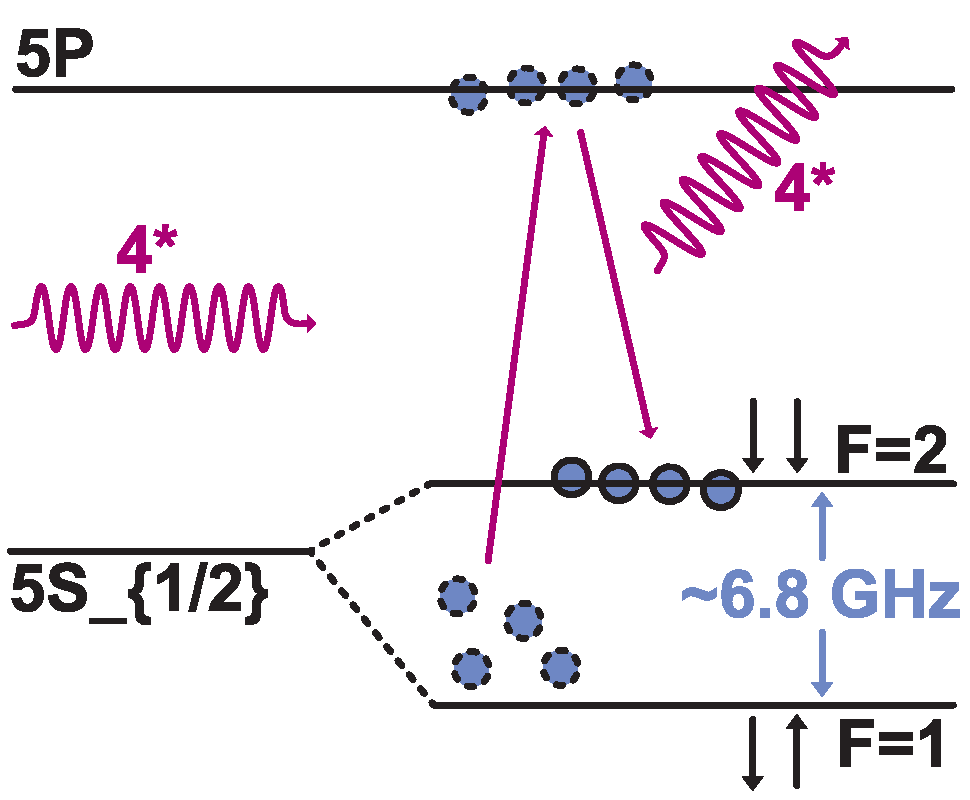
\includegraphics[width=0.9\textwidth]{pdf/MODR/pumping-decay.pdf}}
                \only<2>{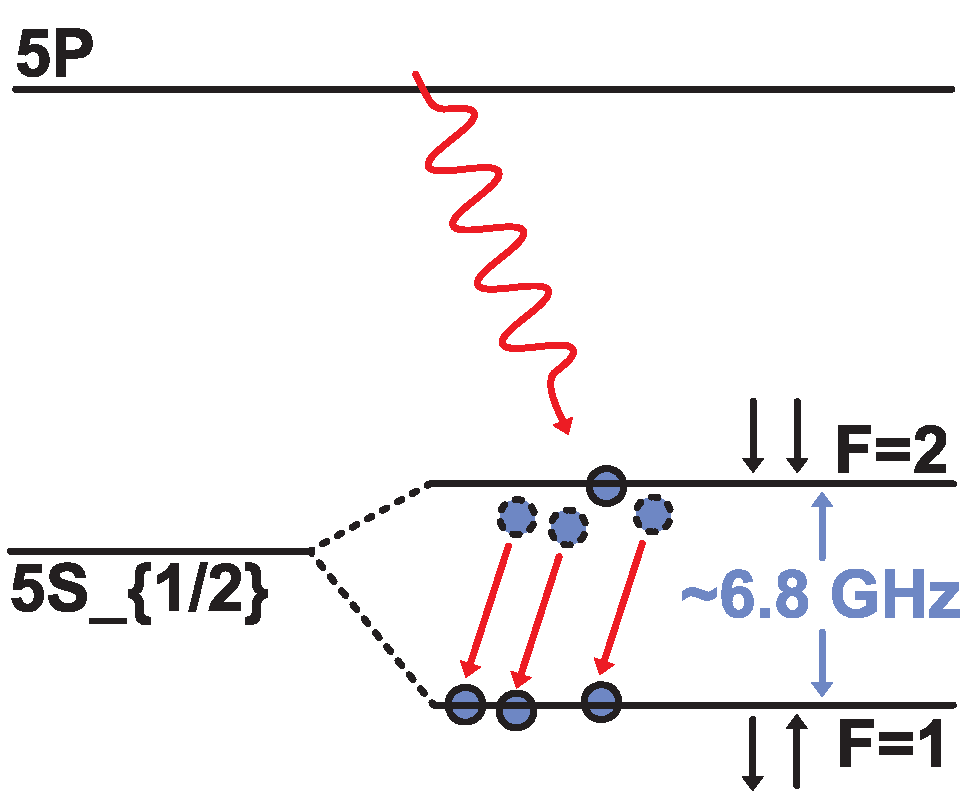
\includegraphics[width=0.9\textwidth]{pdf/MODR/microwave.pdf}}
                \only<3>{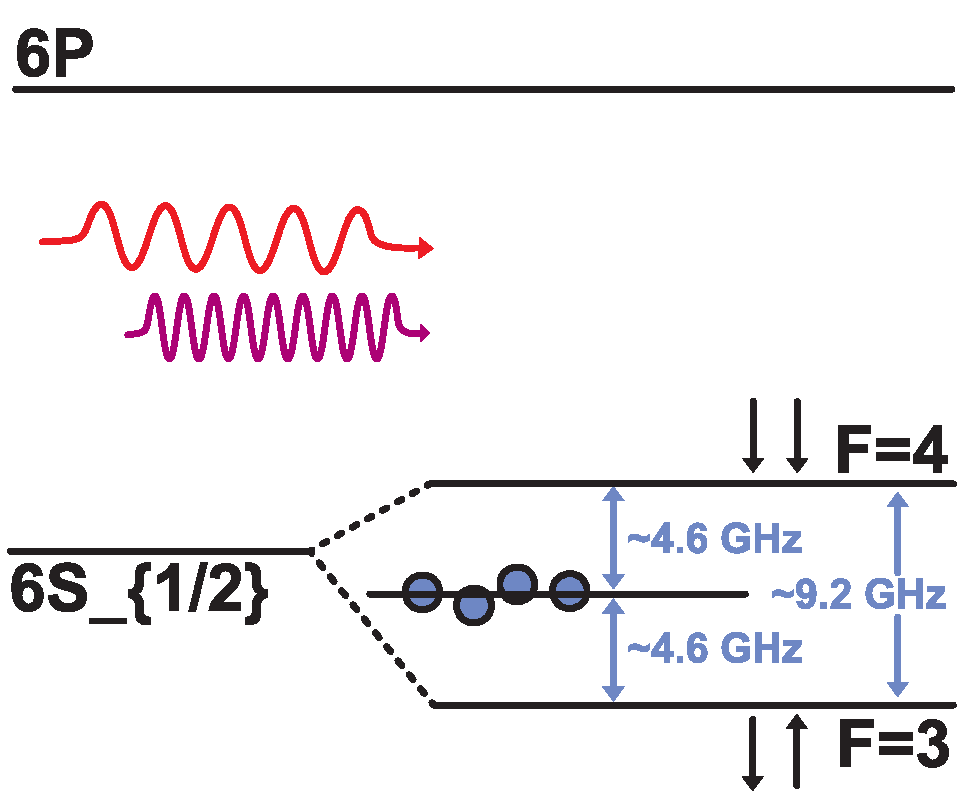
\includegraphics[width=0.9\textwidth]{pdf/MODR/interrogation.pdf}}
            \end{figure}

        \end{column}

        \begin{column}{0.55\textwidth}

            We can distinguish 3 processes:

            \begin{enumerate}
                \item<1-> \textbf<1>{Optical Pumping (Population Inversion)}
                \item<2-> \textbf<2>{Microwave Excitation}
                \item<3-> \textbf<3>{Optical Pumping (Interrogation)}
            \end{enumerate}

        \end{column}

    \end{columns}

    \vspace{10pt}

    \only<1>{
        Ground state population $F=\ket{1}$ gets pumped to $5P$ and then decay to both $F=\ket{1}$ \& $F=\ket{2}$.

        Over time, the population will accumulate in the $F=\ket{2}$ state.
    }
    \only<2>{Microwave tuned at the atomic resonance frequency ($\approx 6.8$ GHz) brings part of the population back to $F=\ket{1}$.}
    \only<3>{Depending on the intensity of the transmitted radiation, \textbf{we can infer if the microwave frequency was in resonance or not}.}

\end{frame}



\begin{frame}{Photodetection}

    At the end of the cell, a photodiode is used to measure the intensity of the transmitted radiation.

    \begin{figure}
        \centering
        \includegraphics[width=0.7\textwidth]{img/MODR-transmission-curve.jpg}
    \end{figure}

    Our target is to stay at the dip of the transmission curve.

\end{frame}



\begin{frame}{Complete Physics Package for a MODR-based CSAC}

    % Previously analyzed components: \textit{Absorption Cell} and \textit{Photocell}.

    \begin{figure}
        \centering
        \includegraphics[width=0.7\textwidth]{img/MODR-physics-package.png}
    \end{figure}

    Other notable components are:

    \begin{itemize}
        \item $^{87}Rb$ Bulb: high frequency radiation source.
        \item $^{85}Rb$ Filter cell: because of overlapping hyperfine levels, it filters out the unwanted transitions frequencies from the lamp.
        \item Microwave cavity: enhances the interaction between radiation and atoms.
    \end{itemize}

\end{frame}


\begin{frame}{Design bottleneck}

    \textit{\dots goal of developing an ultra-miniaturized, low-power, atomic time and frequency reference units\dots}

    \vspace{10pt}

    In case of a MODR-based CSAC, we can recognize multiple problematic areas:

    \begin{itemize}
        \item \textbf{Size}: microwave cavity imposes a low limit ($L_{min} = \frac{c}{2f_{transition}} \approx 2.2cm$).
        \item \textbf{Power consumption}: high ($\approx 10W$) due to thermal stabilization ($\approx 70\%$ of the total).
        \item \textbf{Optical instabilities}: internal wall gas collision\footnotemark[1], Zeeman effects\footnotemark[1], Stark shifts.
    \end{itemize}

    \footnotetext[1]{More on this in the "Extra slides" section.}

\end{frame}


% \begin{frame}{Microwave Cavity}
%     The microwave cavity is used to enhance the interaction between the microwave radiation and the atoms.
%     The cavity is tuned to the atomic resonance frequency.
% \end{frame}